\chapter{Penambangan Data}
\label{ch:penambangan}

Bab ini akan membahas deskripsi data, penyiapan data, dan eksplorasi data dengan menggunakan data \textit{real}

\section{Deskripsi data}
\label{sec:descdat}

Data yang digunakan adalah data yang memiliki format \textit{Comma Separated Value} dengan nama file ''data\_real.csv``. Data ini didapatkan dengan menjalankan kueri pada Kode~\ref{kode:kumpuldatareal} di \textit{platform} bernama \textit{Google BigQuery}. Kueri yang ada akan mengembalikan tabel yang berisi empat kolom dan memiliki 330.781 baris. Data ini diambil dalam rentang waktu 1 Januari 2024 sampai 31 Desember 2024. Sebagai gambaran Tabel~\ref{tab:sepuluhreal} merupakan sepuluh baris pertama dari data yang akan digunakan.

\begin{lstlisting}[language=SQL, caption=Kode untuk mengumpulkan data \textit{real}, label=kode:kumpuldatareal]

SELECT date, client, t.technology, count(t.technology) as jumlah
FROM `httparchive.crawl.pages`, UNNEST(technologies) as t 
WHERE date BETWEEN "2019-01-01" and "2024-12-31"
GROUP BY t.technology, date, client
    
\end{lstlisting}
\begin{table}[H]
\centering
\caption{Sepuluh Baris pertama dari data \textit{real}}
\label{tab:sepuluhreal}
\begin{tabular}{|l|l|l|r|}
\hline
date & client & technology & jumlah \\ \hline
2024-04-01 & desktop & gunicorn & 12.370 \\ \hline
2024-04-01 & desktop & Iterable & 131 \\ \hline
2024-04-01 & desktop & AntV G2 & 946 \\ \hline
2024-04-01 & desktop & Rocketfy & 1 \\ \hline
2024-11-01 & desktop & Platform.sh & 16.634 \\ \hline
2024-11-01 & desktop & Brimble & 2 \\ \hline
2024-10-01 & desktop & Tawk.to & 202.669 \\ \hline
2024-10-01 & desktop & One.com & 92.276 \\ \hline
2024-10-01 & desktop & Bootstrap Table & 8.180 \\ \hline
2024-10-01 & desktop & Saleor & 8 \\ \hline
\end{tabular}
\end{table}

Kolom-kolom tersebut adalah sebagai berikut:
\begin{enumerate}
    \item \textit{date} yang memiliki tipe data \textit{date}. Kolom ini berisi waktu pengetesan dilakukan.

    \item \textit{client} yang memiliki tipe data \textit{string}. Kolom ini berisi perangkat yang digunakan untuk melakukan tes kepada halaman \web. Kolom ini memiliki dua \textit{value} yaitu \desktop dan \mobile.

    \item \textit{technology} yang memiliki tipe data \textit{string}. Kolom ini berisi nama-nama teknologi yang digunakan oleh halaman \web dalam pembuatan atau pengembangan halaman \web tersebut. Kolom ini merupakan elemen dari \textit{array technologies}.

    \item \textit{jumlah} yang memiliki tipe data \textit{integer}. Kolom ini berisi jumlah penggunaan setiap teknologi.
\end{enumerate}

\section{Penyiapan data}
\label{sec:penyiapan}

Data yang telah didapatkan kemudian disiapkan agar lebih mudah dalam melakukan analisis. Salah satu cara yang dapat dilakukan adalah dengan melakukan pembersihan data. Pada data ini ditemukan beberapa baris yang mengalami kesalahan saat proses penarikan data. Sehingga data yang dihasilkan menjadi tidak jelas. Contoh dari masalah ini dapat dilihat pada Tabel~\ref{tab:kesalahan}. Untuk mengatasi masalah ini maka baris yang mengalami kesalahan tadi akan dihapus dari data. Hal ini dilakukan karena jumlah data yang mengalami kesalahan tidak mencapai 10 \% dari total seluruh data. 

\begin{table}[H]
\centering
\caption{Contoh kesalahan saat penarikan data.}
\label{tab:kesalahan}
\begin{tabular}{|l|l|l|r|}
\hline
date & client & technology & jumlah \\ \hline
2022-09-01 & desktop & 2022 & 2 \\ \hline
2019-05-01 & desktop & 255); & 1 \\ \hline
2019-11-01 & mobile & 255); border-style: none; margin: 0px; border-radius: 0px; padding: 0px; & 1 \\ \hline
2020-12-01 & mobile & b) => (a.length > b.length ? a : b)1.7.2 & 1 \\ \hline
2020-11-01 & mobile & yeah & 1 \\ \hline
\end{tabular}
\end{table}


Setelah data dibersihkan, kemudian data diubah ke dalam pivot tabel untuk lebih mudah dalam melakukan eksplorasi. Hal ini bertujuan agar jumlah penggunaan setiap teknologi untuk setiap bulan dapat dengan mudah didapatkan. Tabel~\ref{tab:tabelpivot} adalah tabel pivot yang telah dibuat dan menunjukkan jumlah penggunaan untuk masing-masing teknologi setiap bulannya. Selain jumlah penggunaan setiap teknologi untuk setiap bulanya tabel ini juga memiliki kolom jumlah yang merupakan jumlah penggunaan semua teknologi untuk setiap bulannya.

\begin{table}[H]
\centering
\caption{Tabel pivot untuk mengetahui jumlah penggunaan teknologi setiap bulan}
\label{tab:tabelpivot}
\begin{tabular}{lllll}
\hline
\multicolumn{1}{|c|}{date} & \multicolumn{1}{l|}{Bootstrap} & \multicolumn{1}{l|}{Google Analytics} & \multicolumn{1}{l|}{Google Font API} & \multicolumn{1}{l|}{...} \\ \hline
\multicolumn{1}{|l|}{2019-01-01} & \multicolumn{1}{l|}{10.333.295} & \multicolumn{1}{l|}{27.675.700} & \multicolumn{1}{l|}{15.906.025} & \multicolumn{1}{l|}{...} \\ \hline
\multicolumn{1}{|l|}{2019-02-01} & \multicolumn{1}{l|}{9.989.325} & \multicolumn{1}{l|}{26.912.725} & \multicolumn{1}{l|}{15.522.950} & \multicolumn{1}{l|}{...} \\ \hline
\multicolumn{1}{|l|}{2019-03-01} & \multicolumn{1}{l|}{9.960.270} & \multicolumn{1}{l|}{26.805.405} & \multicolumn{1}{l|}{15.518.165} & \multicolumn{1}{l|}{...} \\ \hline
\multicolumn{1}{|l|}{2019-04-01} & \multicolumn{1}{l|}{11.872.205} & \multicolumn{1}{l|}{31.344.745} & \multicolumn{1}{l|}{18.993.060} & \multicolumn{1}{l|}{...} \\ \hline
\multicolumn{1}{|l|}{2019-05-01} & \multicolumn{1}{l|}{12.341.080} & \multicolumn{1}{l|}{32.557.230} & \multicolumn{1}{l|}{19.735.740} & \multicolumn{1}{l|}{...} \\ \hline
\multicolumn{1}{|l|}{2019-06-01} & \multicolumn{1}{l|}{12.368.135} & \multicolumn{1}{l|}{32.596.160} & \multicolumn{1}{l|}{19.771.645} & \multicolumn{1}{l|}{...} \\ \hline
\multicolumn{1}{|l|}{2019-07-01} & \multicolumn{1}{l|}{13.182.590} & \multicolumn{1}{l|}{34.160.625} & \multicolumn{1}{l|}{21.019.160} & \multicolumn{1}{l|}{...} \\ \hline
\multicolumn{1}{|l|}{2019-08-01} & \multicolumn{1}{l|}{13.146.940} & \multicolumn{1}{l|}{34.057.865} & \multicolumn{1}{l|}{20.922.670} & \multicolumn{1}{l|}{...} \\ \hline
\multicolumn{1}{|l|}{2019-09-01} & \multicolumn{1}{l|}{13.116.225} & \multicolumn{1}{l|}{33.929.805} & \multicolumn{1}{l|}{20.620.630} & \multicolumn{1}{l|}{...} \\ \hline
\multicolumn{1}{|l|}{2019-10-01} & \multicolumn{1}{l|}{13.081.440} & \multicolumn{1}{l|}{33.779.350} & \multicolumn{1}{l|}{20.555.285} & \multicolumn{1}{l|}{...} \\ \hline
\multicolumn{1}{|l|}{...} & \multicolumn{1}{l|}{...} & \multicolumn{1}{l|}{...} & \multicolumn{1}{l|}{...} & \multicolumn{1}{l|}{...} \\ \hline
\end{tabular}
\end{table}

Setelah data disiapkan hal yang dapat dilakukan selanjutnya adalah melakukan eksplorasi data seperti melihat perkembangan sepuluh teknologi yang paling banyak digunakan untuk semua perangkat, perkembangan sepuluh teknologi yang paling banyak digunakan untuk perangkat \mobile dan \desktop, dan melihat perkembangan beberapa teknologi yang nampaknya populer.

\section{Eksplorasi Data}
\label{sec:eksplor}

\subsection{Perkembangan sepuluh teknologi yang paling banyak digunakan di semua perangkat.}
\label{subsec:perkembangansepuluhteknologi}

Hal pertama yang akan dilakukan adalah melihat perkembangan sepuluh teknologi yang paling banyak digunakan untuk membangun atau mengembangkan halaman \web. Proses ini dilakukan dengan cara mengelompokkan data berdasarkan teknologinya dan menghitung jumlah penggunaan untuk setiap teknologi. Data yang sudah dikelompokkan kemudian diurutkan mulai dari teknologi yang jumlah penggunaannya paling banyak. Setelah diurutkan, kemudian sepuluh teknologi yang memiliki jumlah penggunaan paling banyak akan dianalisis lebih lanjut. Sepuluh teknologi tersebut dapat dilihat pada Tabel~\ref{tab:sepuluhteknologipopulerreal}. Terlihat bahwa teknologi yang paling banyak digunakan untuk mengembangkan atau membangun halaman \web adalah \textit{jQuery}.

\begin{table}[H]
\centering
\caption{Sepuluh teknologi dengan jumlah penggunaan paling banyak}
\label{tab:sepuluhteknologipopulerreal}
\begin{tabular}{|c|r|}
\hline
technology & jumlah \\ \hline
jQuery & 1.635.240.294 \\ \hline
Google Analytics & 1.266.635.371 \\ \hline
PHP & 1.155.199.795 \\ \hline
Google Font API & 969.323.383 \\ \hline
Open Graph & 931.262.211 \\ \hline
MySQL & 776.720.413 \\ \hline
WordPress & 728.930.962 \\ \hline
core-js & 713.142.531 \\ \hline
jQuery Migrate & 691.494.400 \\ \hline
Bootstrap & 636.813.294 \\ \hline
\end{tabular}
\end{table}

Kemudian sepuluh teknologi yang paling banyak digunakan ini divisualisasikan perkembangannya. Agar dapat divisualisasikan dengan mudah, maka pekerjaan ini diselesaikan dengan membuat tabel pivot. Tabel pivot seperti pada Tabel~\ref{tab:tabelpivot} berguna agar dapat mengetahui jumlah penggunaan setiap teknologi dalam setiap bulan selama lima tahun. Hasil visualisasi terhadap sepuluh teknologi yang paling banyak digunakan dapat dilihat pada Gambar~\ref{fig:sepuluhteknologireal}.
\begin{figure}[H]
    \centering
    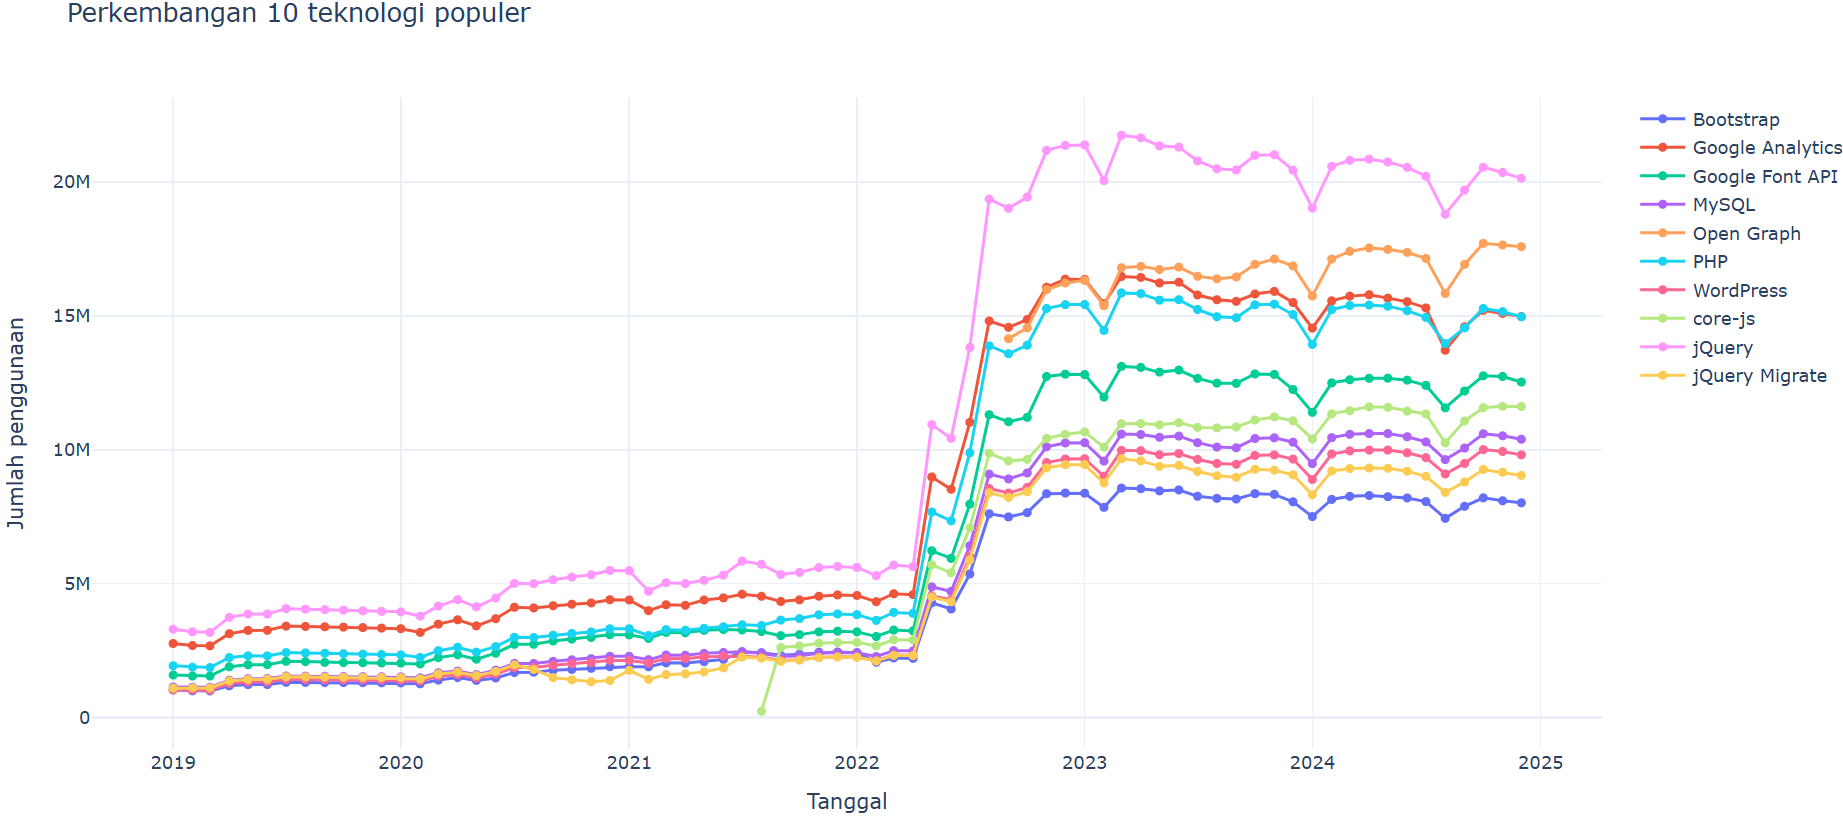
\includegraphics[width=0.7\linewidth]{Gambar/Perkembangan sepuluh real.png}
    \caption{Perkembangan sepuluh teknologi yang paling banyak digunakan membangun \web}
    \label{fig:sepuluhteknologireal}
\end{figure}

Visualisasi yang dihasilkan menunjukkan adanya peningkatan jumlah penggunaan untuk semua teknologi. Terlihat bahwa \textit{core-js} adalah teknologi yang baru masuk sebagai teknologi yang paling banyak digunakan mulai dari Agustus 2021 namun langsung menjadi teknologi terbanyak dipakai urutan ke--6 di bulan selanjutnya. Selain \textit{core-js} ada juga teknologi \textit{Open Graph} yang baru muncul di bulan September 2022 dan langsung menempati urutan ketiga sebagai teknologi yang paling banyak digunakan dalam membangun dan mengembangkan \web yang kemudian menyalip \textit{Google Analytics} pada bulan Maret 2023.

Hasil yang didapatkan dinilai kurang proporsional karena agar perbandingan yang dilakukan lebih proporsional, maka visualisasi diubah menjadi visualisasi berdasarkan persentase penggunaan teknologi bukan lagi berdasarkan jumlah penggunaan. Hal ini dilakukan karena total jumlah penggunaan untuk semua teknologi setiap bulannya tidak sama sehingga agar lebih proporsional. Hasil visualisasi berdasarkan persentase penggunaan ini dapat dilihat pada Gambar~\ref{fig:persentasereal}.

Terlihat adanya penurunan persentase penggunaan untuk semua teknologi yang paling banyak digunakan. Penurunan paling rendah terjadi untuk teknologi \textit{jQuery Migrate} pada bulan November 2020. yang hanya dipakai sebanyak 0,02017\%. Penurunan pada setiap teknologi juga terpengaruh dari jumlah penggunaannya yang semakin tinggi setiap bulan nya.  

\begin{figure}[H]
    \centering
    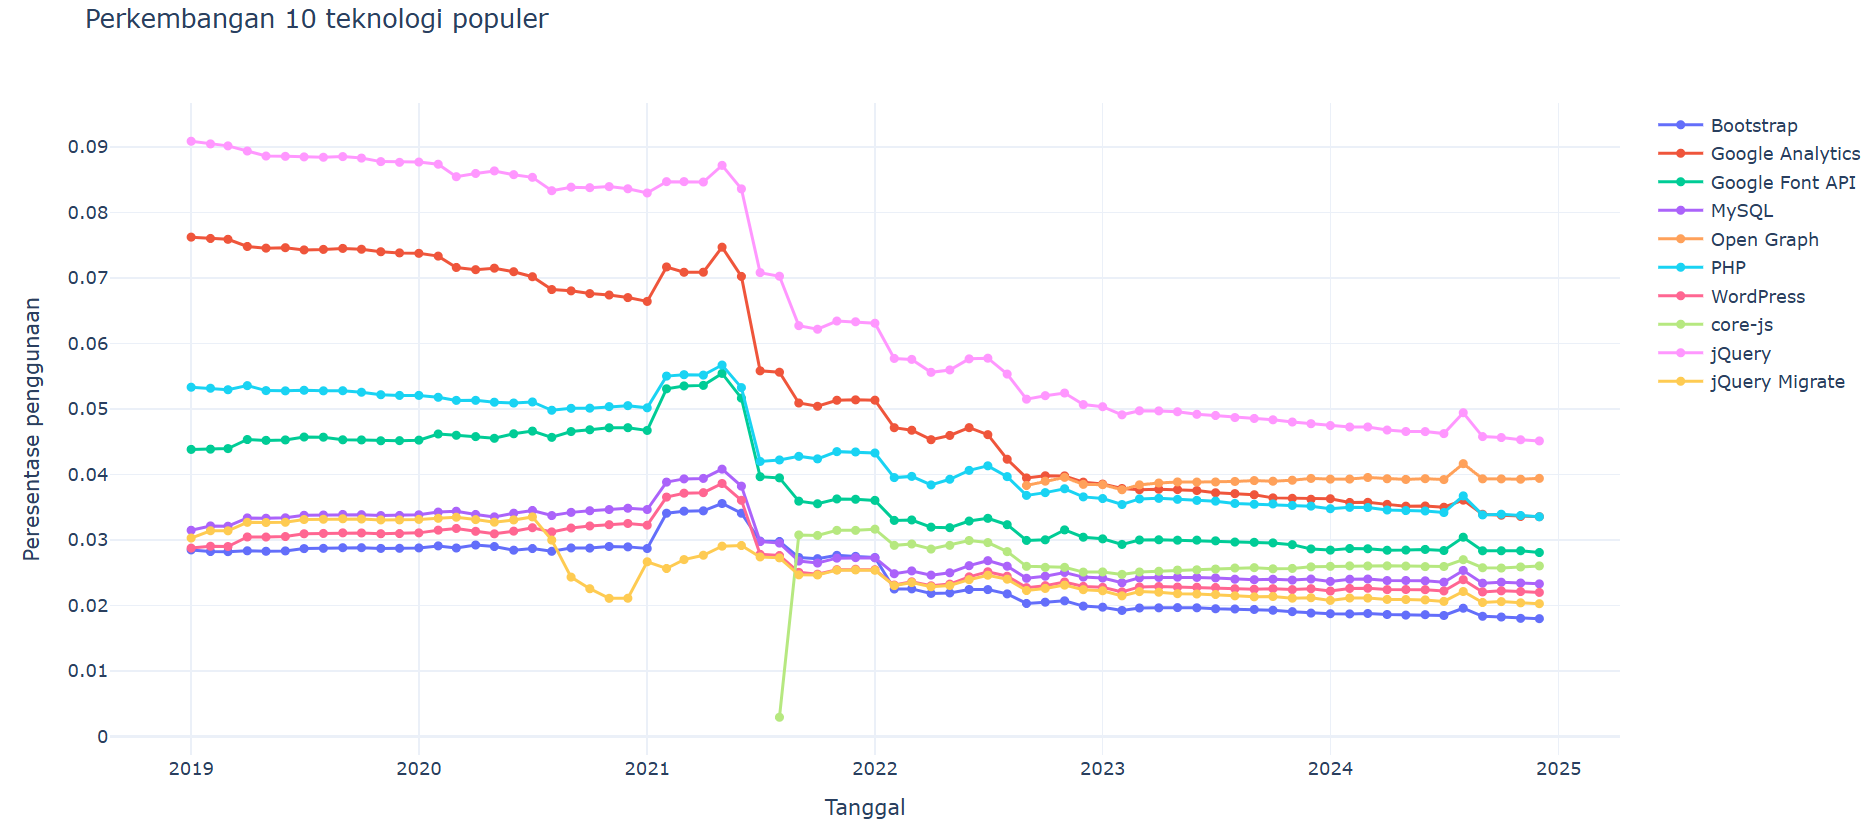
\includegraphics[width=0.7\linewidth]{Gambar/Perkembangan persentase penggunaan real.png}
    \caption{Perkembangan persentase penggunaan dari sepuluh teknologi yang paling banyak digunakan}
    \label{fig:persentasereal}
\end{figure}

\subsection{Perkembangan sepuluh teknologi yang paling banyak digunakan di perangkat \desktop dan \mobile.}
\label{subsec:perkembangansepuluhteknologimobile}

Data yang didapatkan merupakan data yang berasal dari dua perangkat yang berbeda yaitu \mobile dan \desktop. Pada bagian ini yang akan dilihat adalah perkembangan sepuluh teknologi yang paling banyak digunakan pada masing-masing perangkat. Perangkat pertama yang akan ditinjau adalah perangkat \mobile. Metode yang digunakan masih sama yaitu mencari terlebih dahulu sepuluh teknologi yang paling banyak digunakan pada perangkat \mobile. Setelah dikelompokkan dan diurutkan, sepuluh teknologi yang paling banyak digunakan pada perangkat \mobile dapat dilihat pada Tabel~\ref{tab:sepuluhteknologimobilereal}. Terlihat bahwa sepuluh teknologi yang populer di perangkat \mobile masih sama dengan yang terdapat pada Tabel~\ref{tab:sepuluhteknologipopulerreal}.

\begin{table}[H]
\centering
\caption{Sepuluh teknologi dengan jumlah penggunaan paling banyak pada perangkat \mobile}
\label{tab:sepuluhteknologimobilereal}
\begin{tabular}{|c|r|}
\hline
technology & jumlah \\ \hline
jQuery & 907.815.523 \\ \hline
Google Analytics & 694.557.335 \\ \hline
PHP & 649.411.801 \\ \hline
Google Font API & 541.528.239 \\ \hline
Open Graph & 520.578.213 \\ \hline
MySQL & 435.952.366 \\ \hline
WordPress & 410.439.160 \\ \hline
core-js & 392.176.760 \\ \hline
jQuery Migrate & 388.203.382 \\ \hline
Bootstrap & 355.050.603 \\ \hline
\end{tabular}
\end{table}

Setelah sepuluh teknologi yang paling banyak digunakan pada perangkat \mobile didapatkan kemudian divisualisasikan dengan cara yang sama seperti pada bagian \ref{subsec:perkembangansepuluhteknologi}. Visualisasi pertama dilakukan berdasarkan jumlah penggunaan teknologi. Kemudian dilanjutkan dengan visualisasi berdasarkan persentase penggunaannya. Untuk visualisasi berdasarkan jumlah penggunaannya hasilnya dapat dilihat pada Gambar~\ref{fig:sepuluhmobilereal}. Terlihat bahwa perkembangannya semakin meningkat untuk semua teknologi, namun untuk teknologi \textit{jQuery} jumlah penggunaan pada perangkat mobile memiliki rentang yang lebih tinggi. 

\begin{figure}[H]
    \centering
    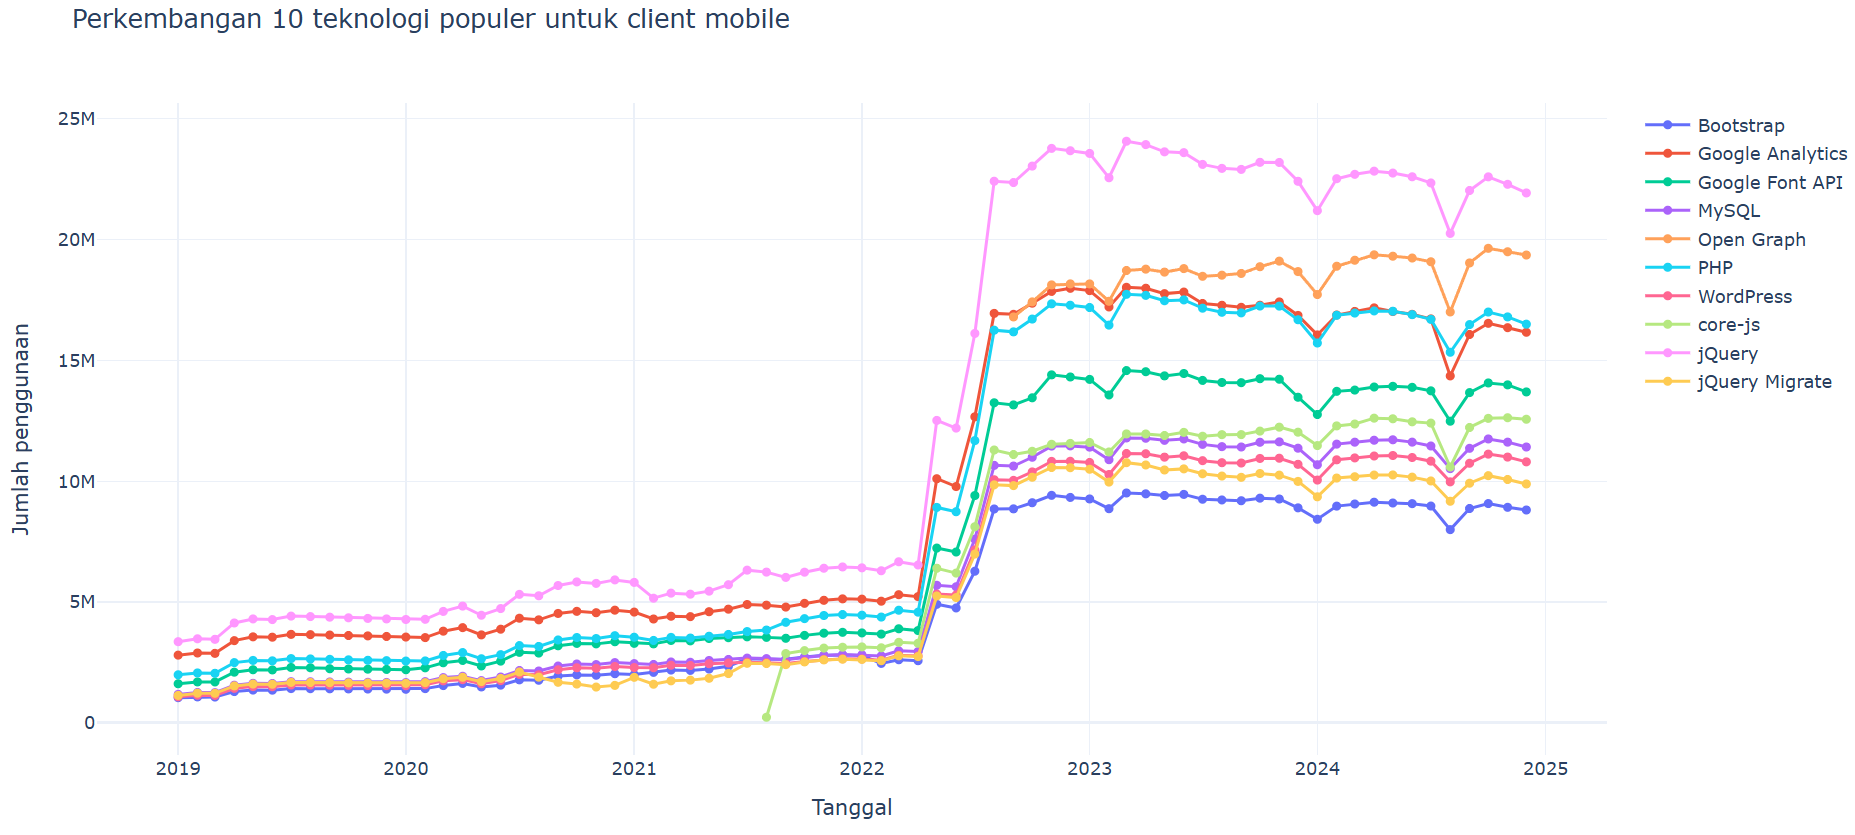
\includegraphics[width=0.7\linewidth]{Gambar/perkembanganmobilereal.png}
    \caption{Perkembangan sepuluh teknologi paling banyak diggunakan pada perangkat \mobile}
    \label{fig:sepuluhmobilereal}
\end{figure}

Setelah melihat perkembangan jumlah penggunaan, hal yang selanjutnya akan ditinjau adalah persentase penggunaan teknologi pada perangkat \mobile. Hasil visualisasi untuk persentase penggunaan ini dapat dilihat pada Gambar~\ref{fig:persentasemobilereal} Terlihat bahwa visualisasi yang dihasilkan tidak berbeda jauh dengan Gambar~\ref{fig:persentasereal}. Yang berbeda adalah rentang persentasenya lebih rendah.

\begin{figure}[H]
    \centering
    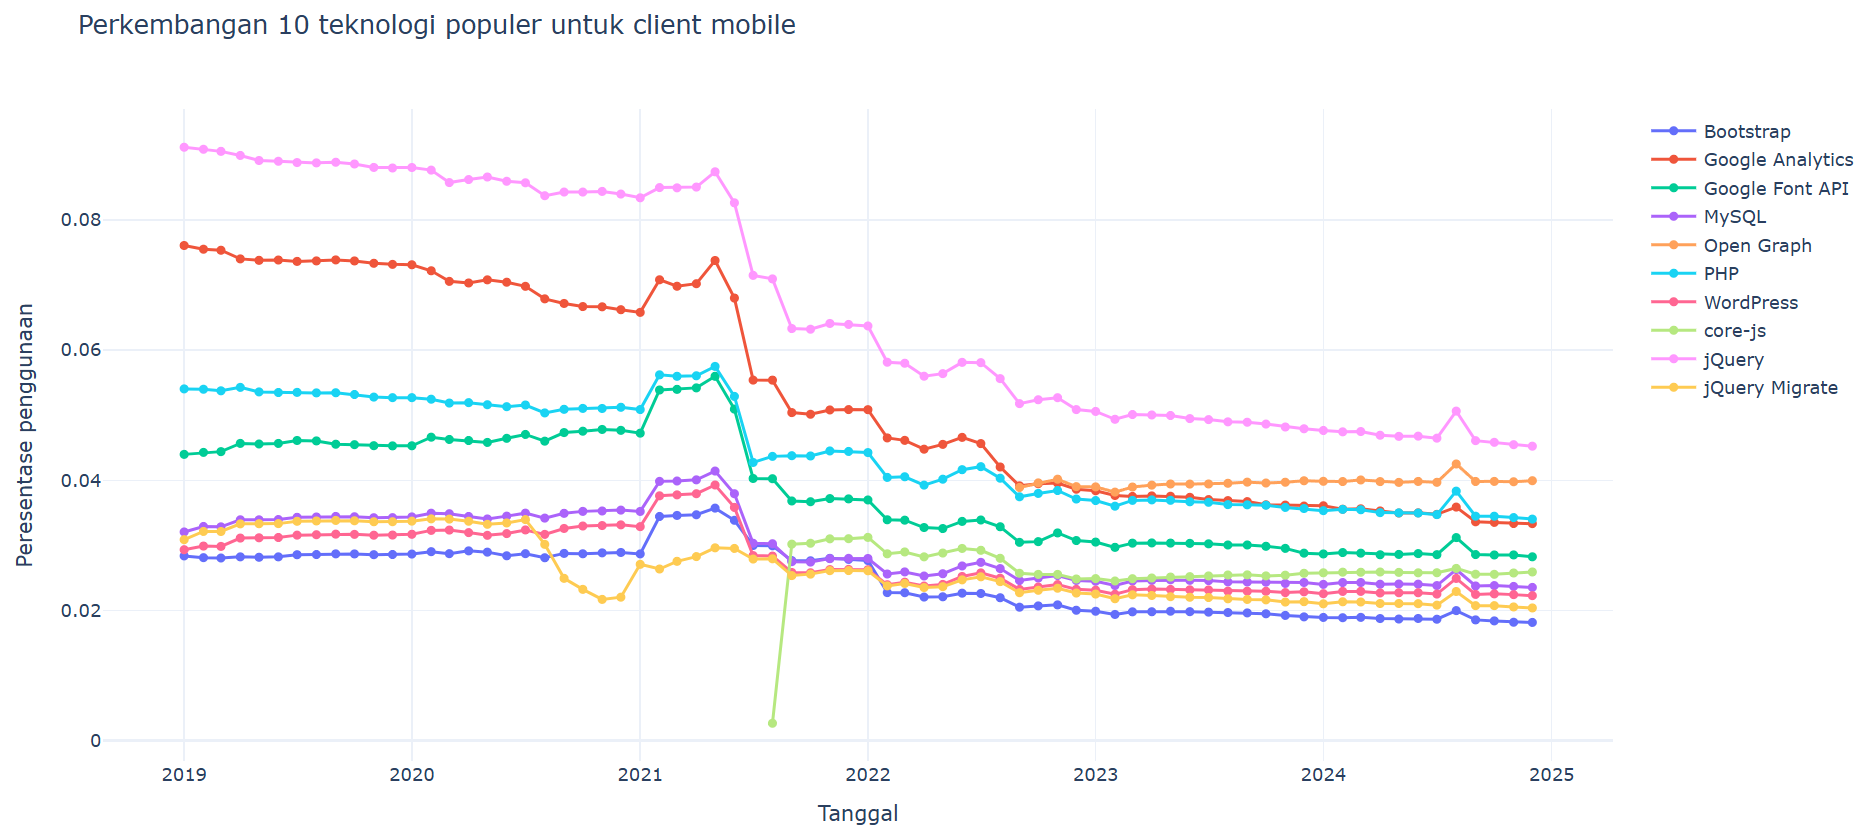
\includegraphics[width=0.7\linewidth]{Gambar/persentasemobilereal.png}
    \caption{Perkembangan persentase penggunaan teknologi pada perangkat \mobile}
    \label{fig:persentasemobilereal}
\end{figure}

Perangkat selanjutnya yang akan dianalisis adalah perangkat \desktop. Metode yang digunakan pada analisis ini masih sama yaitu dengan mencari sepuluh teknologi yang paling banyak digunakan.  Setelah itu melakukan visualisasi berdasarkan jumlah penggunaan teknologi dan persentase penggunaan teknologi tersebut. Sepuluh teknologi yang paling banyak digunakan pada perangkat \desktop dapat dilihat pada Tabel~\ref{tab:sepuluhdesktopreal}. Terlihat adanya teknologi baru yang masuk yaitu \textit{Google Tag Manager}. Terlihat juga dari jumlah penggunaan masing-masing teknologi lebih rendah daripada jumlah penggunaan teknologi pada perangkat \mobile. 

\begin{table}[H]
\centering
\caption{Sepuluh teknologi yang paling banyak digunakan pada perangkat \desktop}
\label{tab:sepuluhdesktopreal}
\begin{tabular}{|l|l|}
\hline
technology & jumlah \\ \hline
jQuery & 745.620.826 \\ \hline
Google Analytics & 585.708.398 \\ \hline
PHP & 513.344.386 \\ \hline
Google Font API & 435.039.011 \\ \hline
Open Graph & 410.683.998 \\ \hline
MySQL & 344.462.488 \\ \hline
WordPress & 322.822.568 \\ \hline
core-js & 320.965.771 \\ \hline
jQuery Migrate & 307.386.712 \\ \hline
Google Tag Manager & 288.083.449 \\ \hline
\end{tabular}
\end{table}

Hasil visualisasi berdasarkan jumlah penggunaan dari sepuluh teknologi yang paling banyak digunakan pada perangkat \desktop dapat dilihat pada Gambar~\ref{fig:sepuluhdesktopreal}. Terlihat bagwa pada perangkat \desktop juga terdapat peningkatan pada semua teknologi. Namun untuk teknologi \textit{Google Tag Manager} perkembangannya sangat tidak stabil. Hal ini terlihat dari jumlah penggunaan yang naik dan turun secara signifikan. Pada perangkat \desktop juga teknologi \textit{Open Graph} baru mulai digunakan pada bulan September 2022.

\begin{figure}[H]
    \centering
    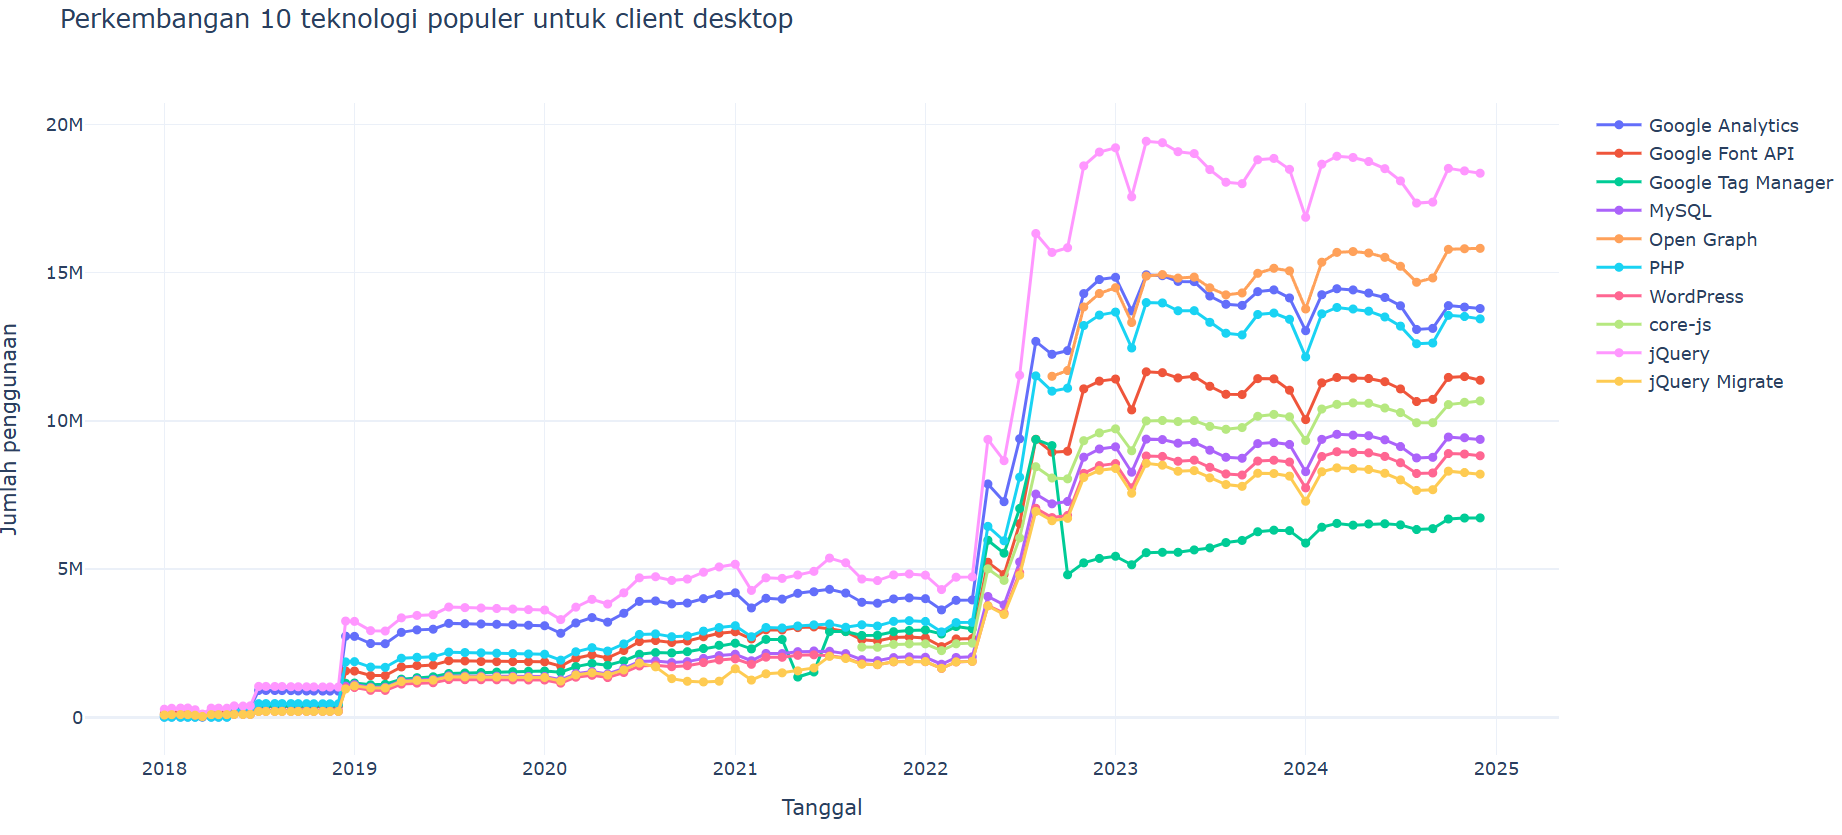
\includegraphics[width=0.7\linewidth]{Gambar/Perkembangan desktop real.png}
    \caption{Perkembangan sepuluh teknologi paling banyak diggunakan pada perangkat \desktop}
    \label{fig:sepuluhdesktopreal}
\end{figure}

Selain dari jumlah penggunaannya, visualisasi juga dilakukan berdasarkan persentase penggunaan dari sepuluh teknologi yang paling banyak digunakan. Hasil visualisasi berdasarkan persentase penggunaan ini dapat dilihat pada Gambar~\ref{fig:persentasedesktopreal}. Terlihat adanya perbedaan yang sangat signifikan di antara semua teknologi, namun kembali stabil pada Mei 2018. Persentase penggunaan untuk semua teknologi mengalami penurunan. Teknologi yang paling tidak stabil perkembangannya adalah \textit{Google Tag Manager}. Visualisasi ini juga menunjukkan untuk teknologi \textit{jQuery} persentase penggunaan pada bulan Januari 2018 -- Mei 2018 merupakan persentase penggunaan paling tinggi kemudian untuk teknologi \textit{Google Analytic} pada rentang waktu yang sama merupakan persentase penggunaan yang paling rendah.

\begin{figure}[H]
    \centering
    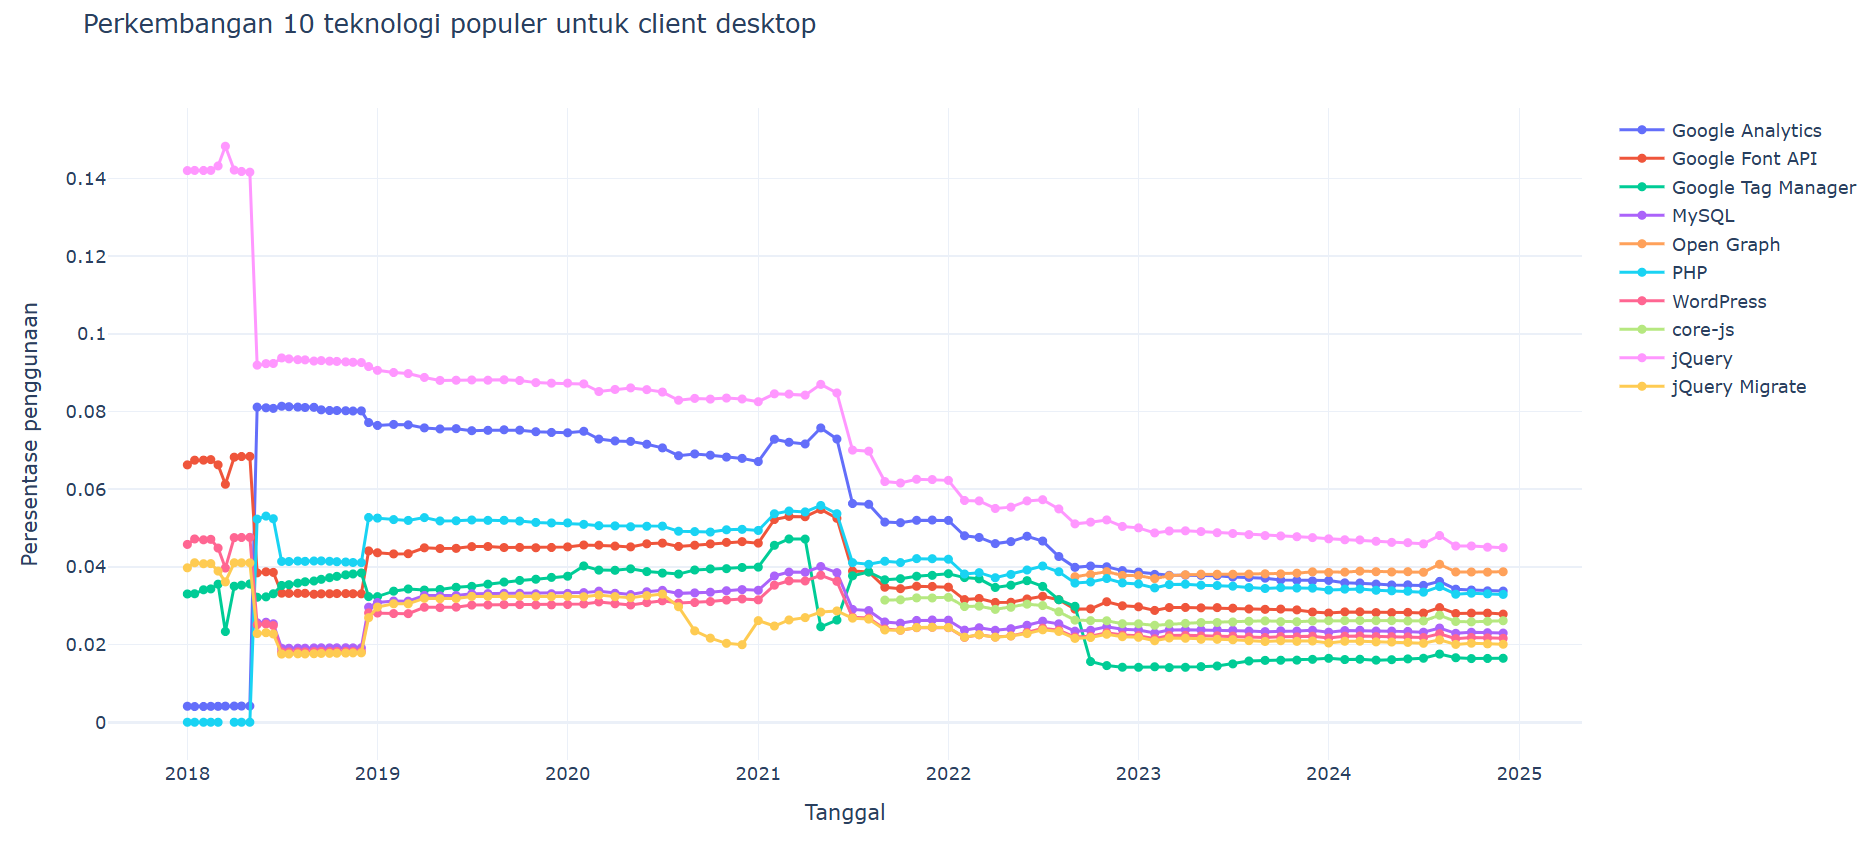
\includegraphics[width=0.7\linewidth]{Gambar/Perkembangan persentase desktop real.png}
    \caption{Perkembangan persentase penggunaan teknologi pada perangkat \desktop }
    \label{fig:persentasedesktopreal}
\end{figure}

\subsection{Perbandingan teknologi yang nampak populer}
\label{subsec:teknologipopulerlain}

Bagian ini akan membandingkan beberapa teknologi yang paling banyak digunakan dengan beberapa teknologi yang nampak populer dalam semua perangkat. Teknologi-teknologi ini diambil dari daftar teknologi pengembangan \web yang populer dari halaman \url{https://www.geeksforgeeks.org/top-web-development-trends/#most-popular-web-development-technologies}. Perbandingan akan dilakukan terhadap teknologi yang dipakai pada \textit{back-end} maupun \textit{front-end} dalam pengembangan \web.

\subsubsection{\textit{PHP} dengan \textit{Node.js}}
\label{subsubsec:phpnode}

\textit{PHP} dan \textit{Node.js} merupakan dua teknologi yang dipakai pada bagian \textit{back-end} dalam pengembangan \web. Node.js merupakan teknologi yang cukup populer. Namun dari data yang dapatkan seperti yang terlihat pada Gambar~\ref{fig:phpnode} teknologi \textit{Node.js} tidak digunakan sebanyak teknologi \textit{PHP}, sehingga \textit{Node.js} tidak masuk ke dalam daftar teknologi yang paling banyak digunakan. Perbedaan jumlah penggunaan juga sangat besar terlihat dari penggunaan \textit{PHP} yang berkisar di antara 20 juta penggunaan sedangkan \textit{Node.js} hanya berkisar di antara 600.000 penggunaan.

Sementara itu dari segi persentase penggunaan menunjukkan hal yang sama. Terlihat pada Gambar~\ref{fig:phpnodepersen} bahwa persentase penggunaan dari teknologi PHP lebih tinggi jika dibandingkan dengan teknologi \textit{Node.js}. Terlihat bahwa penggunaan teknologi \textit{PHP} berkisar antara 0.035-0.055\% sedangkan teknologi \textit{Node.js} penggunaannya tidak lebih dari 0.01\%. Kemungkinan penyebab teknologi \textit{Node.js} kurang banyak diminati oleh pengembang \web adalah karena \textit{JavaScript} menyediakan banyak varian teknologi yang dapat dipilih oleh pengembang. Sehingga jumlah penggunaannya terbagi ke teknologi dari \textit{JavaScript yang lain.}

\begin{figure}[H]
    \centering
    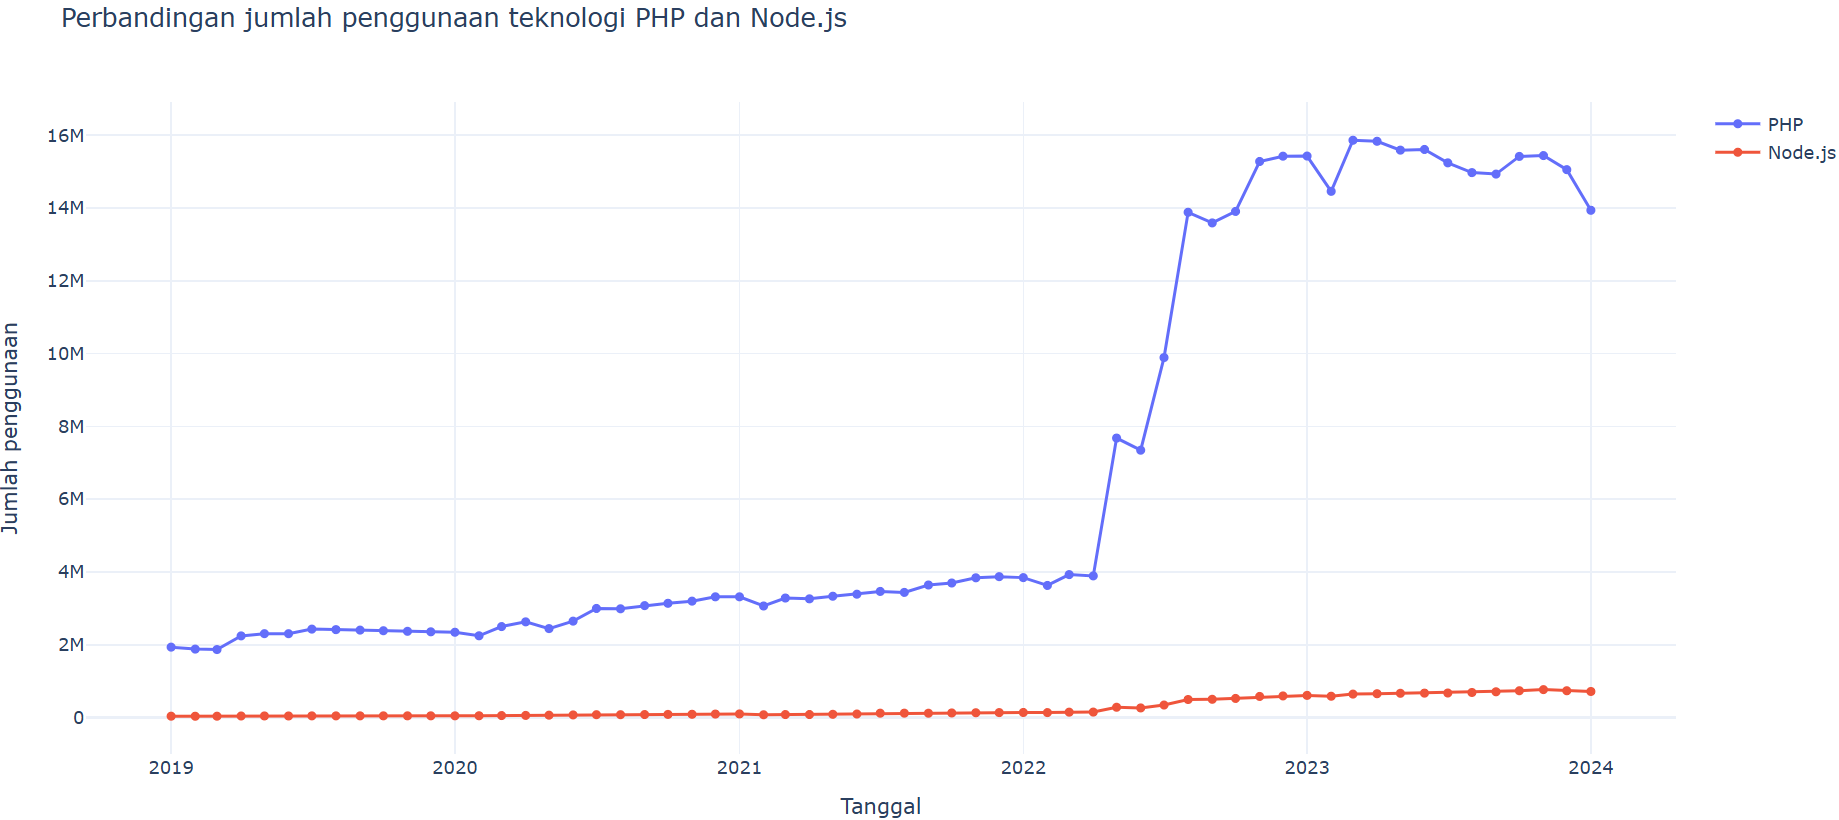
\includegraphics[width=0.7\linewidth]{Gambar/perbandinganphpnode.png}
    \caption{Perbandingan jumlah penggunaan teknologi \textit{PHP} dan \textit{Node.js}}
    \label{fig:phpnode}
\end{figure}

\begin{figure}[H]
    \centering
    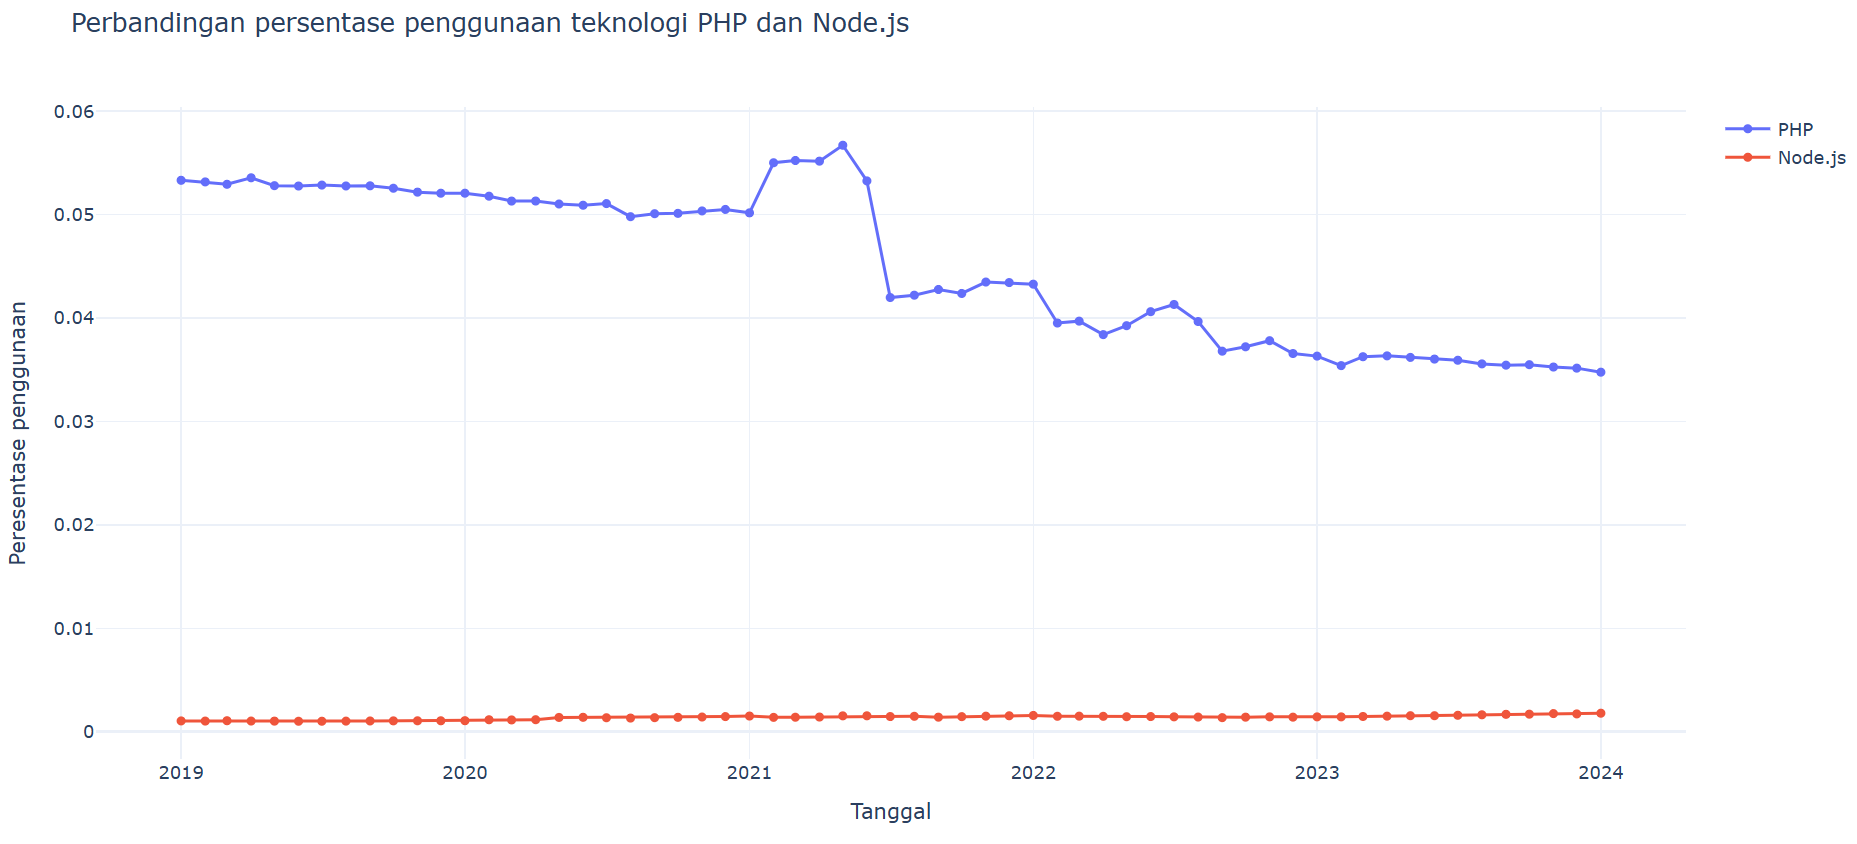
\includegraphics[width=0.7\linewidth]{Gambar/Perbandinganpersentasephpnode.png}
    \caption{Perbandingan persentase penggunaan teknologi \textit{PHP} dan \textit{Node.js}}
    \label{fig:phpnodepersen}
\end{figure}

\subsubsection{\textit{jQuery} dengan \textit{Angular}}
\label{subsubsec:angularjq}

\textit{jQuery} dan \textit{Angular} merupakan teknologi yang dipakai pada bagian \textit{front-end} dalam pengembangan \web. Angular merupakan teknologi yang cukup populer, tetapi berdasarkan data yang didapatkan, \textit{Angular} memiliki jumlah penggunaan yang sangat kecil seperti yang dapat dilihat pada Gambar~\ref{fig:angularjq}. Terlihat bahwa jumlah halaman \web yang menggunakan teknologi \textit{Angular} tidak lebih dari 200.000. Hal ini juga berpengaruh terhadap persentase penggunaan seperti yang dapat dilihat pada Gambar~\ref{fig:angularjqpersen}. Teknologi \textit{Angular} tidak memiliki persentase yang lebih dari 0.01\%. Kemungkinan penyebab rendahnya jumlah penggunaan teknologi \textit{Angular} adalah karena pengembang tidak terlalu tertarik untuk menggunakan \textit{Angular}.

\begin{figure}[H]
    \centering
    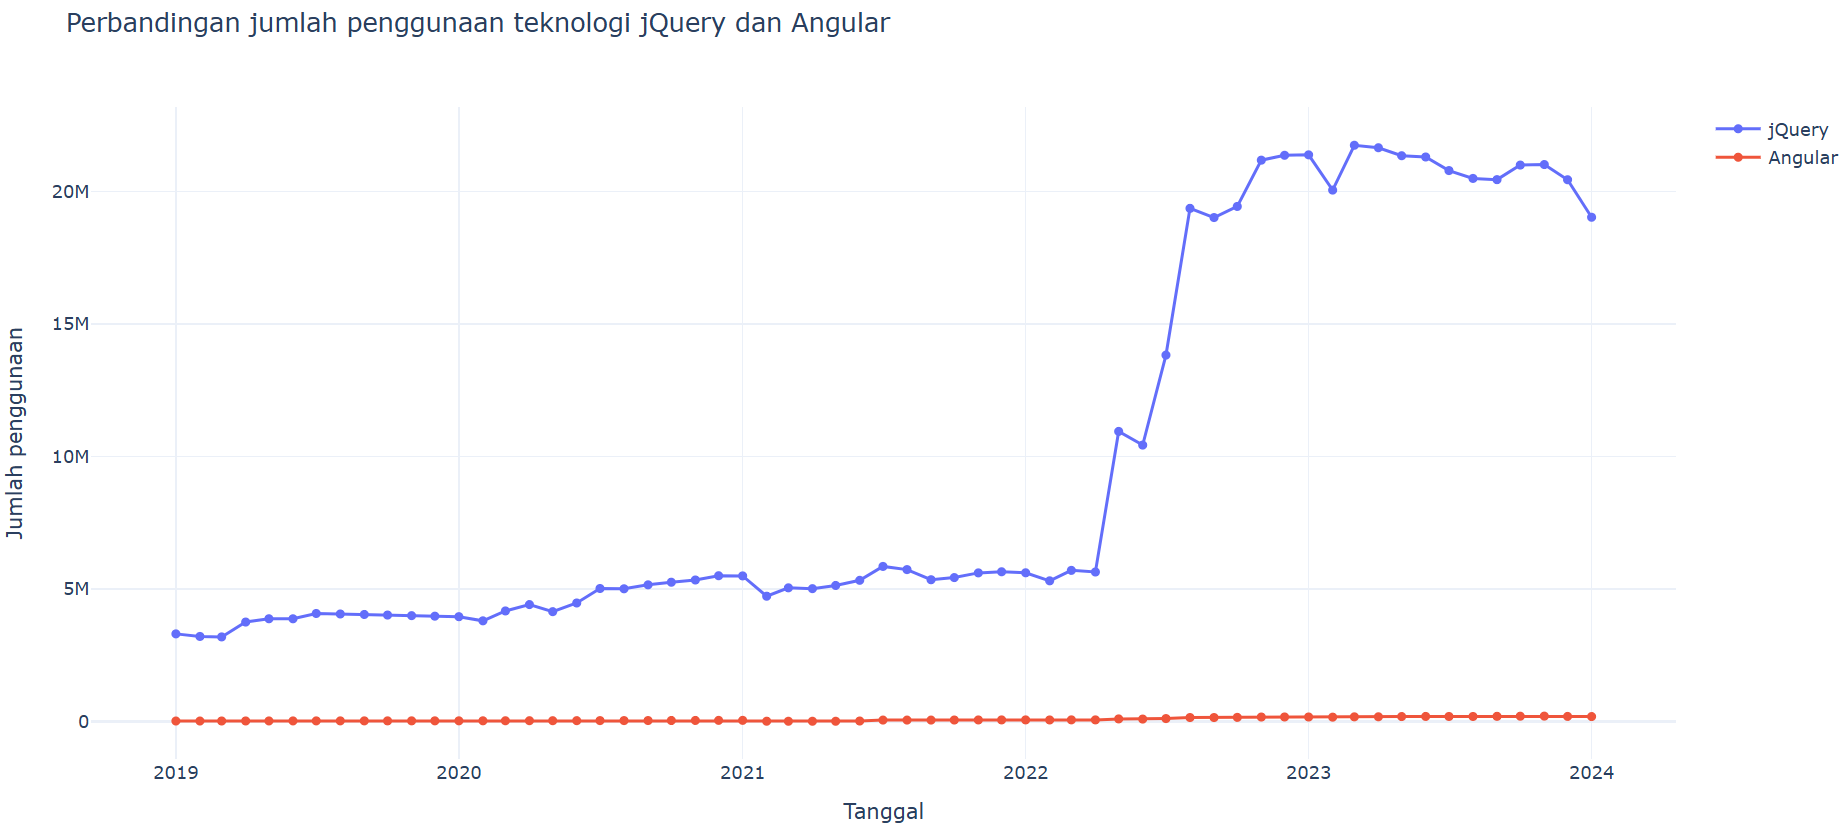
\includegraphics[width=0.7\linewidth]{Gambar/perbandinganangularjq.png}
    \caption{Perbandingan jumlah penggunaan teknologi \textit{jQuery} dan \textit{Angular}}
    \label{fig:angularjq}
\end{figure}

\begin{figure}[H]
    \centering
    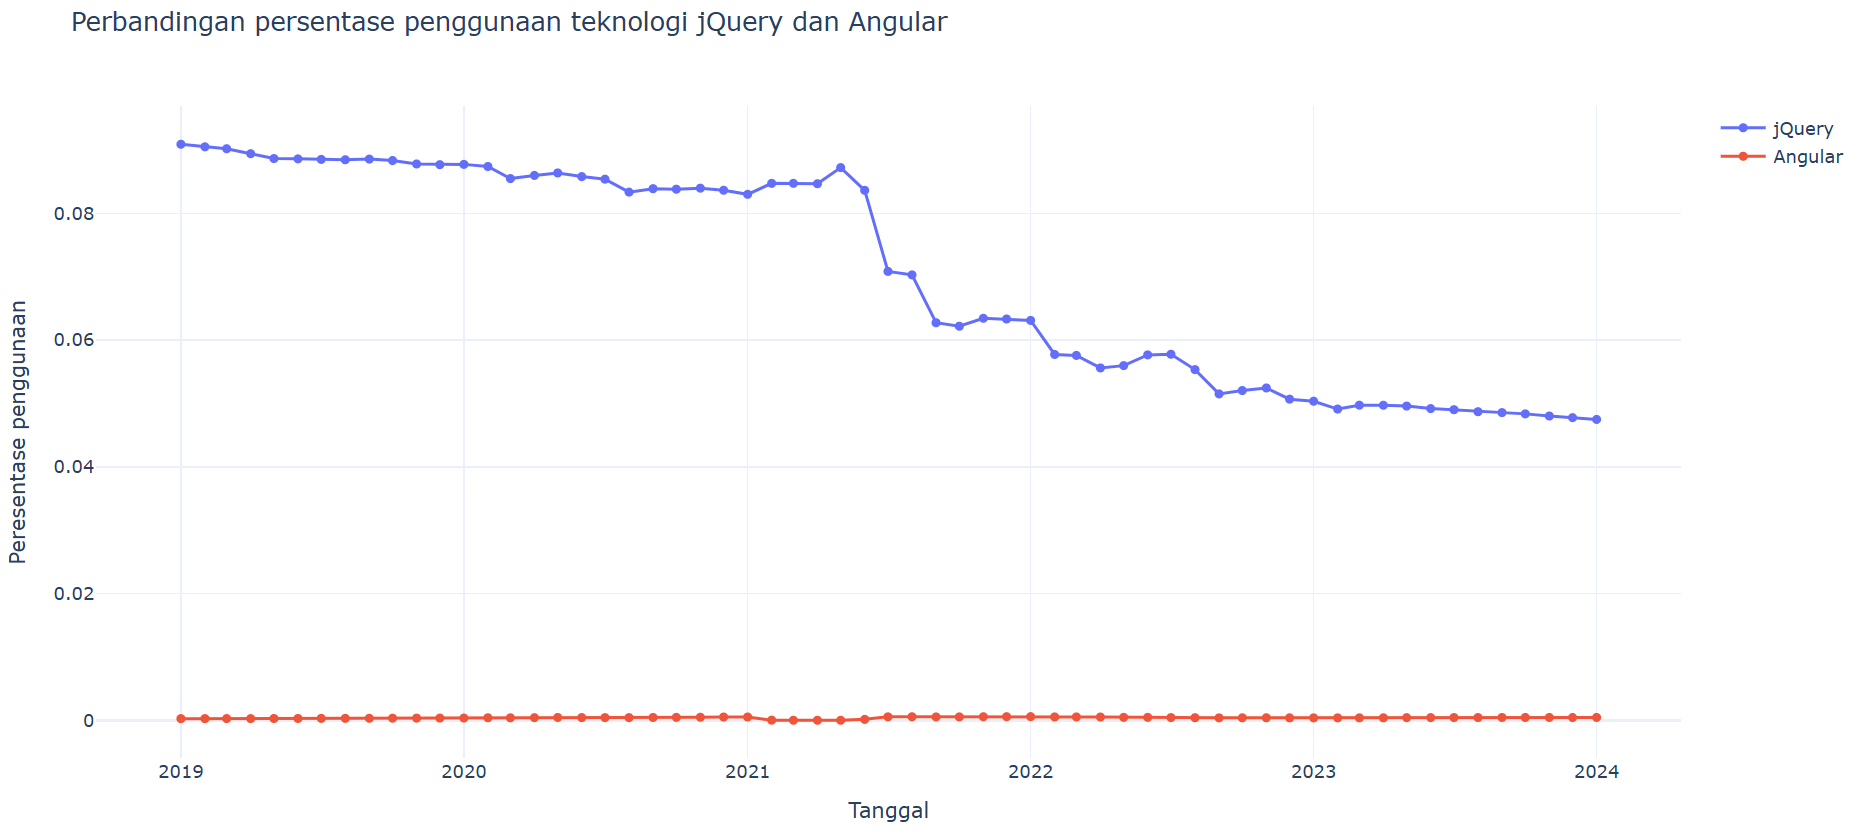
\includegraphics[width=0.7\linewidth]{Gambar/angularjqpersen.png}
    \caption{Perbandingan persentase penggunaan teknologi \textit{jQuery} dan \textit{Angular}}
    \label{fig:angularjqpersen}
\end{figure}